\section{Други домаћи задатак}
По угледу на пример 4.3 из документа Предавање 2, генерисати по $N=500$ одбирака из двеју дводимензионалних класа.
\begin{enumerate}[a)]
\item На дијаграму приказати одбирке
\item Генерисати геометријско место тачака са константном вредношћу функција густина вероватноће па их приказати на дијаграму у простору облика.
\item Испројектовати Бајесов класификатор минималне грешке и на дијаграму, заједно са одбирцима, скицирати класификациону линију, па проценити вероватноћу грешке.
\item Поновити претходну тачку за неки други класификатор по избору.
\item а класе облика генерисаних у претходним тачкама, испројектовати Валдов секвенцијални тест, па скицирати зависност броја потребних одбирака од усвојене вероватноће грешке првог, односно другог типа.
\end{enumerate}

\subsection{Генерисање одбирака}

За почетак генерисаћемо одбирке двеју дводимензионалних класа чије су функције густине вероватноће у облику бимодалних гаусовских расподела:


$$f_1(X) = P_{11} N(M_{11}, \Sigma_{11}) + P_{12} N(M_{12}, \Sigma_{12})$$
$$f_2(X) = P_{21} N(M_{21}, \Sigma_{21}) + P_{22} N(M_{22}, \Sigma_{22}),$$
при чему вероватноће, средње вредности и коваријационе матрице имају следеће вредности:
$$P_{11} = 0,6,  M_{11} = \begin{bmatrix}
   -1,5\\
   4,5
\end{bmatrix}, 
S_{11} = \begin{bmatrix}
				   3,5 & -1\\
				   -1 & 2,2
				\end{bmatrix},
P_{12} = 0,4,  M_{12} = \begin{bmatrix}
										   -0,5\\
										   0,5
										\end{bmatrix}, 
S_{12} = \begin{bmatrix}
				   1,3 & 0,9\\
			   	0,9 &  2
				\end{bmatrix}
$$				
$$P_{21} = 0,45,  M_{21} = \begin{bmatrix}
   7,5\\
   -3,5
\end{bmatrix}, 
S_{21} = \begin{bmatrix}
				   1,5 & 1,1\\
				   1,1 & 1,5
				\end{bmatrix},
P_{22} = 0,55,  M_{22} = \begin{bmatrix}
										   4\\
										   2
										\end{bmatrix}, 
S_{22} = \begin{bmatrix}
				   3 & -0,8\\
			   	-0,8 &  3
				\end{bmatrix}
$$

За генерисање одбирака коришћене су две функције. Одсечак кода прве функције која је коришћена је дат на одсечку \ref{fun:gausGenerate}. Овде се користи својство да се "обична" Гаусова расподела са варијансама 1 и очекивањем 0 кад се помножи са $\Phi \Lambda^\frac{1}{2}$, при чему су $\Phi$ матрица вектора сопствених вредности и $\Lambda$ матрица сопствених вредности од $S_x$, и на крају дода $M_x$, при чему је $M_x$ математичко очекивање вектора за који хоће да се генерише дата расподела, добије се Гаусова расподела са математичким очекивањем $M_x$ и $S_x$.

\renewcommand{\lstlistingname}{Одсечак кода}%
	
\begin{lstlisting}[caption={Вишеваријабална Гаусова расподела-генерисање},label={fun:gausGenerate}]
function [X] = gausianMultivariateGenerate(Mx, Sx, num_points)
% Generates a matrix whose size is num_points, also it has 
% gausian multivarate distribution with Mx mean and 
% Sx covariance matrix. 

[F, L] = eig(Sx);

n = size(Sx, 1);
X = randn(n, num_points);

for i = 1 : num_points
    X(1:n, i) = F * sqrt(L) * X(1:n, i) + Mx; 
end

end
\end{lstlisting}

Друга коришћена функција је дата у одсечку  \ref{fun:gausGenerateModal}. Она користи својство да је бимодална Гаусова расподела збир две Гаусове са одређеним вероватноћама и тако генерише потребну расподелу. 

\begin{lstlisting}[caption={Вишеваријабална мултимодална Гаусова расподела-генерисање},label={fun:gausGenerateModal}]
function [X] = gausianMultimodalGenerate(P1,P2, M1, M2, S1, S2, num_points)
X = zeros(num_points, 2);
for i = 1 : num_points
    probability = rand(1, 1);
    if (probability < P1)
        X(i, :) = gausianMultivariateGenerate(M1, S1, 1);
    else
        X(i, :) = gausianMultivariateGenerate(M2, S2, 1);
    end
end
end
\end{lstlisting}
Позивањем \emph{gausianMultimodalGenerate} са одговарајућим параметрима за обе класе добија се расподела као на слици \ref{fig:Odbirci}. 
\begin{figure}[htb!]
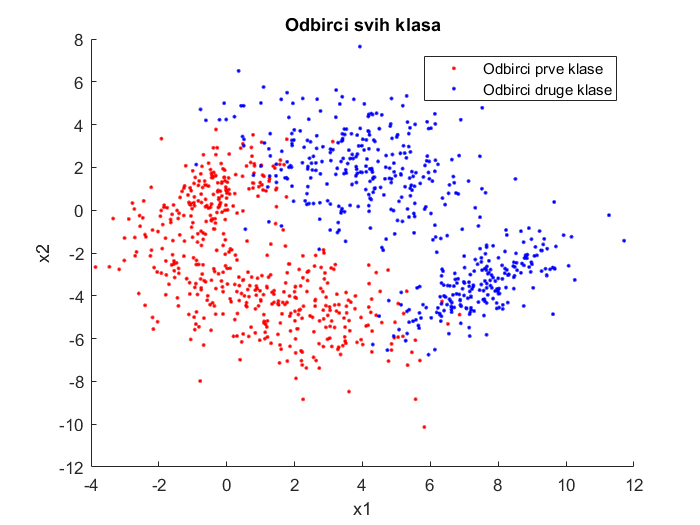
\includegraphics[scale=1]{pictures/2/Odbirci}
\caption{Одбирци}\label{fig:Odbirci}
\end{figure}

\newpage
\subsection{Функција густине вероватноће}
Функција густине вероватноће је израчуната за сваки "део" тако што је за сваку тачку у размаку од $0,1$ у интервалу $[-6, -12]$ на $x$ оси и на интервалу $[-10, 8]$ на $y$ оси позивана функција која је дата одсечком кода \ref{fun:gausMultiModal}. Дата функција густине вероватноће може да се види у \emph{3D} на слици \ref{fig:FGV}. На слици \ref{fig:FGVContour} налазе се геометријска места тачака функције густине вероватноће од сваке класа, и то $0,8 * max(f(X))$, $0,6 * max(f(X))$, $0,4 * max(f(X))$, $0,2 * max(f(X))$. Може да се примети да они делови "класа" који су "оштрији" имају неке вредности које "тупљи" делови немају.

\begin{lstlisting}[caption={Вишеваријабална мултимодална Гаусова расподела-функција густине},label={fun:gausMultiModal}]
function [f] = gausianMultimodal(X, P1, P2, M1, M2, S1, S2)
%GAUSIANMULTIMODAL Calculates multimodal probability density function.
f = P1 * gausianMultivariate(X, M1, S1) + P2 * gausianMultivariate(X, M2, S2); 
end
\end{lstlisting}

\begin{figure}[htb!]
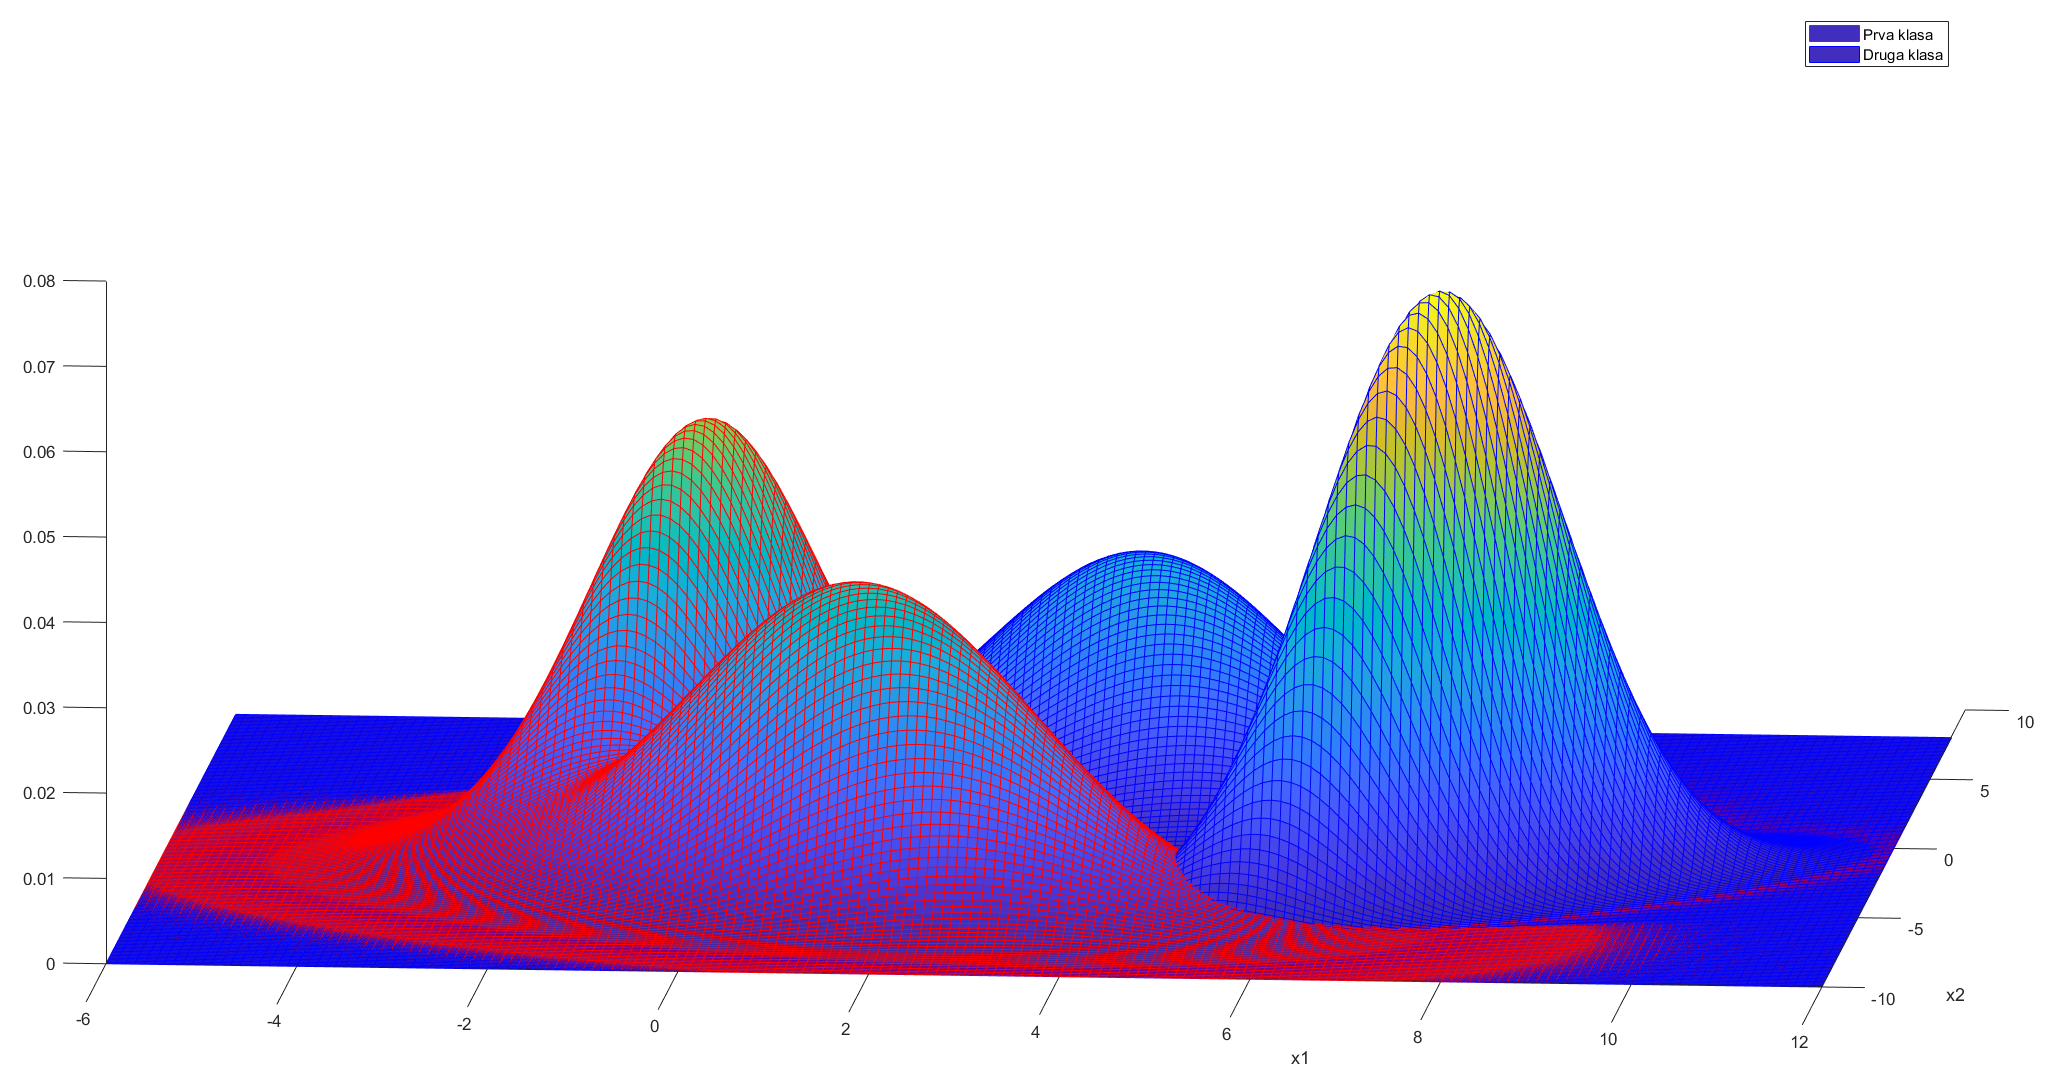
\includegraphics[scale=0.33]{pictures/2/FGV}
\caption{Функције густине вероватноће}\label{fig:FGV}
\end{figure}

\begin{figure}[htb!]
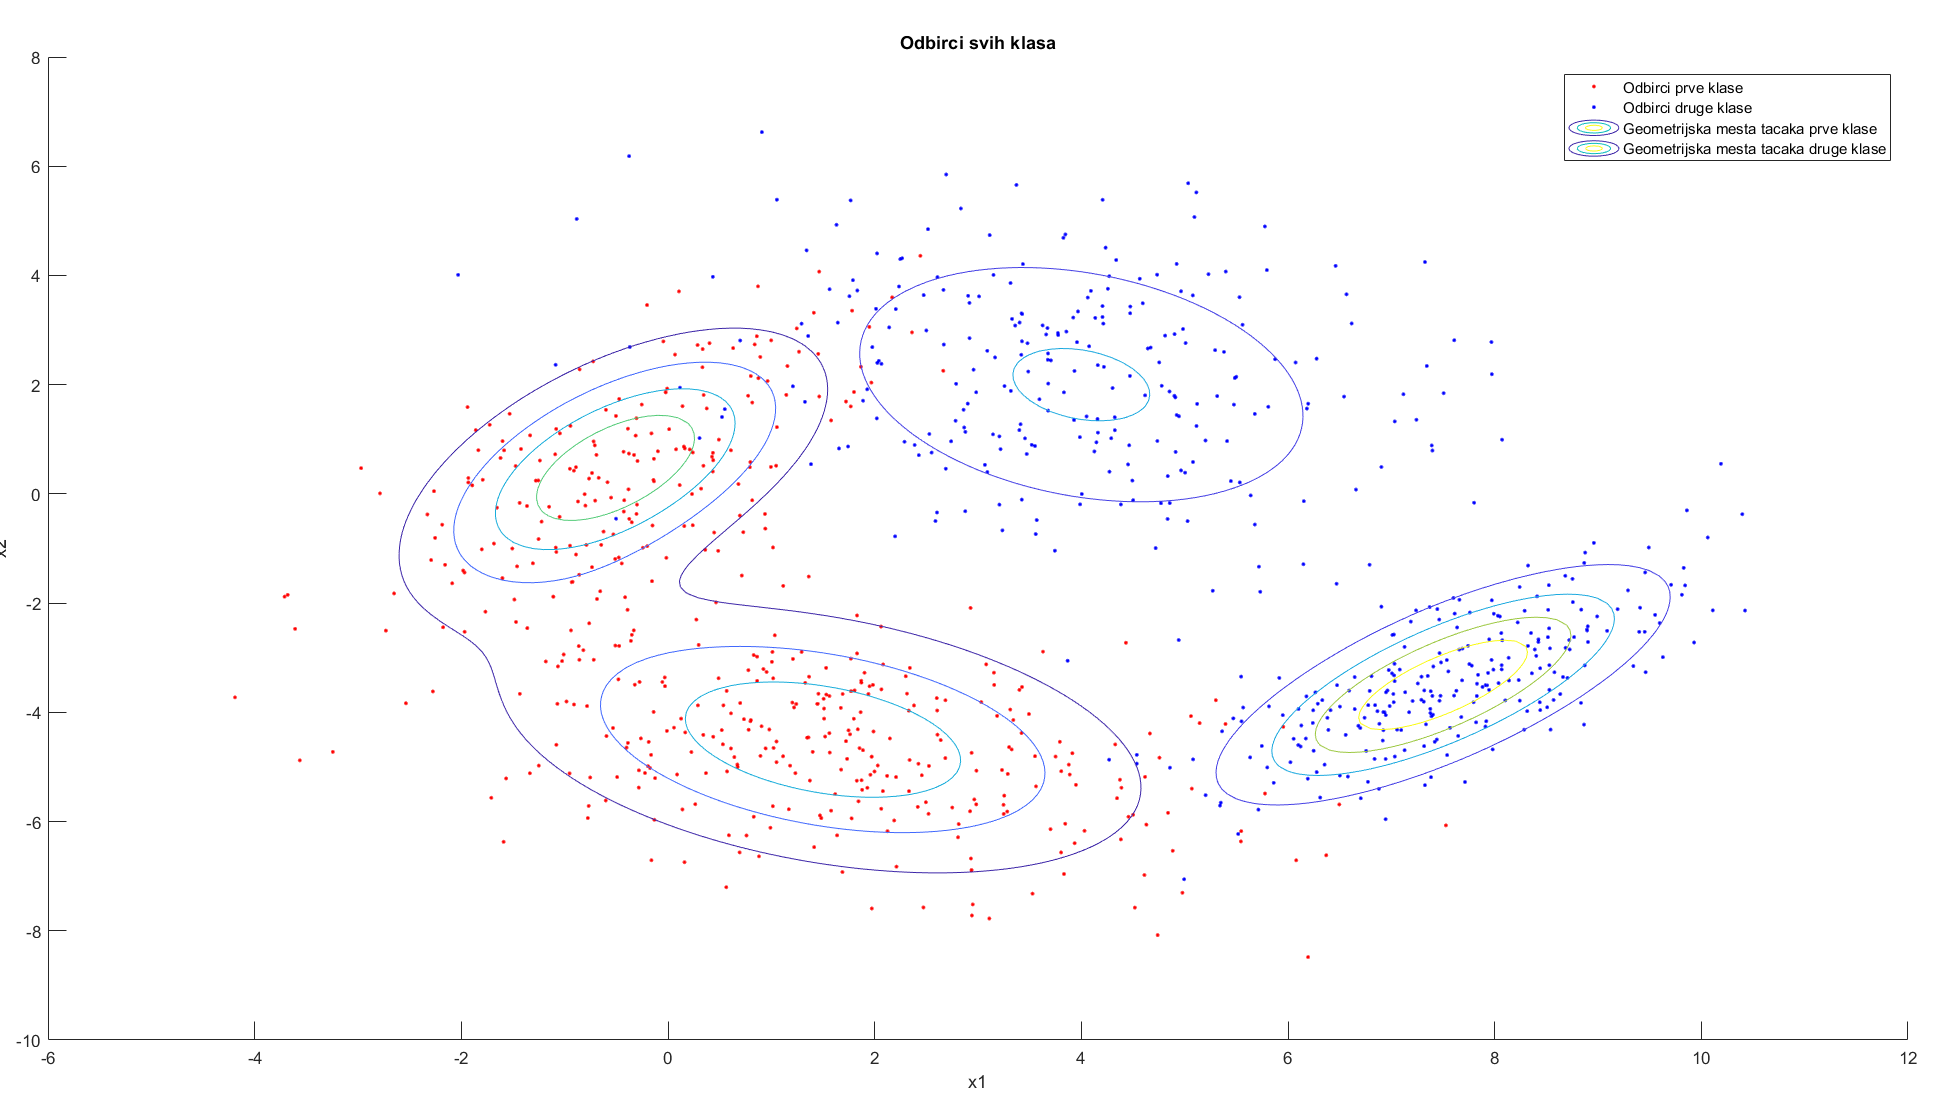
\includegraphics[scale=0.33]{pictures/2/FGVContour}
\caption{Функције густине вероватноће-геометријска места тачака}\label{fig:FGVContour}
\end{figure}
\newpage
\subsection{Бајесов класификатор минималне грешке}
Дати класификатор има следеће правило одлучивања:
$$h(X) = -ln(f_1(X) + ln(f_2(X)) < ln\left( \frac{P_1}{P_2}\right) \implies X \in \omega_1$$
$$h(X) = -ln(f_1(X) + ln(f_2(X)) >ln\left( \frac{P_1}{P_2}\right) \implies X \in \omega_2$$
где су $P_1, P_2$ априорне вероватноће појављивања класа. Како је број генерисаних тачака 500, важи $P_1 = P_2 = 0,5$, стога $h(X)= 0$. Геометријска места тачака, као и дискриминациона функција је дата на слици \ref{fig:Bayes}.

\begin{figure}[htb!]
\centering
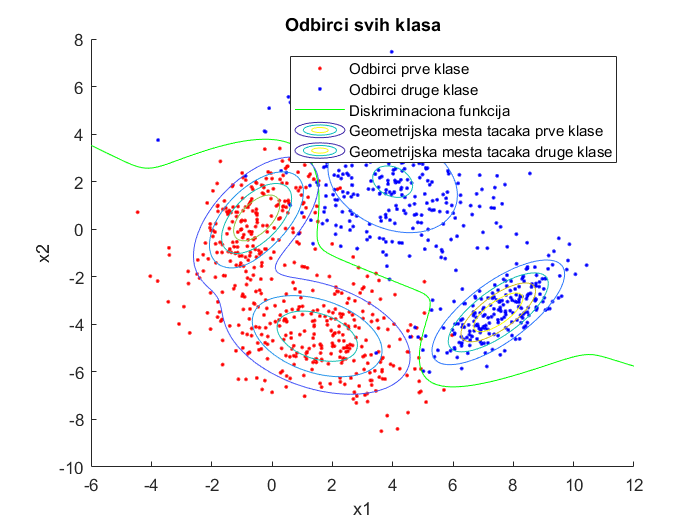
\includegraphics[scale=0.53]{pictures/2/Bayes}
\caption{Функције густине вероватноће, геометријска места тачака и дискриминациона линија}\label{fig:Bayes}
\end{figure}
На одсечку кода \ref{fun:genBayes} је приказано како је генерисана дискриминациона функција.
\begin{lstlisting}[caption={Генерисање дискриминационе функције},label={fun:genBayes}]
X1 = gausianMultimodalGenerate(P11, P12, M11, M12, S11, S12, num_points);
X2 = gausianMultimodalGenerate(P21, P22, M21, M22, S21, S22, num_points);

step = 0.1;
xIt = -6 : step : 12;
yIt = -10 : step : 8;

m = length(xIt);
n = length(yIt);

f1 = zeros(m, n);
f2 = zeros(m, n);
h = zeros(m, n);

[XItGrid, YItGrid] = meshgrid(xIt, yIt);

for i = 1 : m
    for j = 1 : n
        tempInput = [XItGrid(i, j) YItGrid(i, j)]';
        f1(i, j) = gausianMultimodal(tempInput, P11, P12, M11, M12, S11, S12);
        f2(i, j) = gausianMultimodal(tempInput, P21, P22, M21, M22, S21, S22);
        h(i, j) = log(f2(i, j)) - log(f1(i, j));
        
    end
end

f1Max = max(max(f1));
f2Max = max(max(f2));

figure(1);
hold on;    
plot(X1(:, 1), X1(:, 2), 'r.'); 
plot(X2(:, 1), X2(:, 2), 'b.');

xlabel('x1');
ylabel('x2');

title('Odbirci svih klasa');

contour(XItGrid, YItGrid, h, [0 0], 'g');
contour(XItGrid, YItGrid, f1, [0.8 * f1Max f1Max * 0.6 f1Max * 0.4 f1Max * 0.2]);
contour(XItGrid, YItGrid, f2, [0.8 * f2Max f2Max * 0.6 f2Max * 0.4 f2Max * 0.2]);

legend('Odbirci prve klase', 'Odbirci druge klase', 'Diskriminaciona funkcija',...
        'Geometrijska mesta tacaka prve klase', 'Geometrijska mesta tacaka druge klase');

\end{lstlisting}
Вероватноћа грешке првог и другог типа се рачунају по формули:
$$\varepsilon_1 = \int_{L_2} f_1(X)dX, \varepsilon_2 = \int_{L_1}f_2(X)dX,$$
При чему су $L1, L2$ области на које дели дискриминациона функција, при чему је $L1$ она област за коју густина вероватноће припадност класи 1 има већу вредност, за $L2$ обратно.
Пошто интеграл није решив, рачунао се методом правоугаоника (квадара). Функција из одсечка кода \ref{fun:epsilonEst} је имплементација методе правоугаоника(квадара).Вредност грешке првог типа је $3,7\%$ а другог типа је $3,8\%$.

\begin{lstlisting}[caption={Процена грешке},label={fun:epsilonEst}]
function [epsilon1,epsilon2] = errorEstimation(f1, f2, disFunction, num_rows, num_cols, step)
epsilon1 = 0;
epsilon2 = 0;

for i = 1 : num_rows
    for j = 1 : num_cols
        if (disFunction(i, j) < 0)
            epsilon2 = epsilon2+ f2(i, j) * step^2;
        else 
            epsilon1 = epsilon1 + f1(i, j) * step^2;
        end
    end
end

end
\end{lstlisting}

\subsection{Бајесово правило одлучивања минималне цене}
Класификацију ћемог поново извршити, али овога пута помоћу Бајесоовг правила одлучивања минималне цене. Тест је сличан Бајесовом, с тим да одговарајућих коефицијенти кажњавају грешке једног или другог типа, односно "дозвољавају" их. $c_{ij}$ цена одлуке $X \in \omega_i$ кад је заправо $X \in \omega_j$. Условна цена одлуке износи 
$$r_i(X) = c_{i1}q_1(X) + c_{i2}q_2(X),$$ тј.
$$r_1(X) < r_2(X) \implies X \in \omega_1$$
$$r_1(X) > r_2(X) \implies X \in \omega_2$$
Тада априорни ризик добија облик: $r(X) = min(r_1(X), r_2(X))$. Минимизацијом израза добија се:
$$\frac{f_1(X)}{f_2(X)} > \frac{(c_{12}-c_{22})P_2}{(c_{21} - c_{11})P_1} \implies X\in \omega_1$$
$$\frac{f_1(X)}{f_2(X)} < \frac{(c_{12}-c_{22})P_2}{(c_{21} - c_{11})P_1} \implies X\in \omega_2$$
Како је $P_2 = P_1$, и $h(X) = -ln(\frac{f_1(X)}{f_2(X)}$ добија се:
$$h(X) = ln(f_2(X) (c_{12} - c_{22})) - ln(f_1(X)(c_{21} - c_{11})) < 0 \implies X \in \omega_1$$
$$h(X) = ln(f_2(X) (c_{12} - c_{22})) - ln(f_1(X)(c_{21} - c_{11})) >0 \implies X \in \omega_2$$

Ако ставимо  $c_{11} = c_{22} = 0$ постављањем $c_{12}, c_{21}$ на одговарајуће вредности добијамо да се кажњава више одговарајући тип грешке (в. сл. \ref{fig:BayesMinimal}). У случају $c_{12} = 3, c_{21} = 1$ добијамо да је дискриминациона функција примакнута првој класи, што има смисла, јер се кажњава промашај ако је се претпоставило да је прва класа, а треба да је друга. Обратно, важи само за другу класу кад је $c_{21} = 3, c_{12} =1$. Кад је $c_{21}=c_{12}$ тест постаје Бајесов класификатор минималне грешке (што се и види на слици).
Грешке су рачунају истом функцијом као и Бајесов класификатор, при чему у првом случају је грешка прве врсте $0, 072$, а друге $0, 018$, а у другом $0, 017$ односно $0,072$. Претходно је такође логично јер је у првом случају дискриминациона функција близу прве класе и више ће бити погрешно класификованих њених одбирака у другу класу. 


\begin{figure}[htb!]
\centering
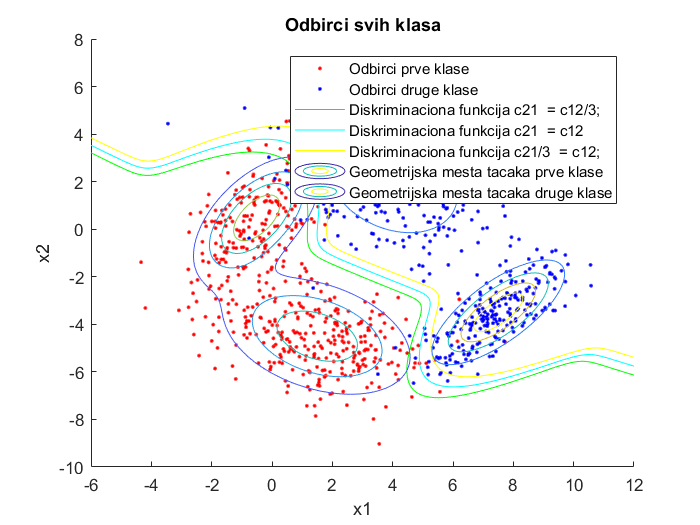
\includegraphics[scale=1]{pictures/2/BayesMinimal}
\caption{Тест минималне цене}\label{fig:BayesMinimal}
\end{figure}
\subsection{Волдов секвенцијални тест}

У претходно обрађеним класификаторима одлука је доношена само на основу информација које тренутно се поседују. Али у многим практичним применама информације стижу секвенцијално и њихов број се увећава. Фамилија секвенцијалних класификатора у озбир узима и претходна мерења. Један од њих је Волдов тест. Он доноси одлуку након коначног броја мерења када вероватноћа грешке спадне на жељене нивое $\varepsilon_1$ и $\varepsilon_2$.

Дефинишемо $s$ који представља негативни логаритам здружене функције густине вероватноће свих мерења и узимамо претпоставку да су оне независне:

$$s_m = -ln\frac{f_1(X_1, ..., X_m)}{f_2(X_1, ..., X_m)} = \sum_{i=1}^m \left( -ln\frac{f_1(X_i)}{f_2(X_i)}\right) = \sum_{i=1}^mh(X_i)$$

Волдов тест функционише:
\begin{enumerate}[1)]
\item $s_m \leq a \implies X \in \omega_1$
\item $a < s_m < b \implies $ узети следеће мерење
\item $s_m \geq b \implies X \in \omega_2$
\end{enumerate}

Границе $a$ и $b$ су директно повезане са $\varepsilon_1$ и $\varepsilon_2$ и износе:
$a=-ln\frac{1-\varepsilon_1}{\varepsilon_2}$, $b =-ln\frac{\varepsilon_1}{1-\varepsilon_2}$

Код који имплементира је одсечак кода \ref{fun:waldoTest}. Можемо да видимо да код понавља $testCases$ пута Валдов тест да би усредњио број итерација неопходан за детекцију класе којој припада јер се насумично узимају тачке из одређене класе $X$. 

\begin{lstlisting}[caption={Одређивање припадностие},label={fun:waldoTest}]
function [classIdx, i] = waldosTest(X, epsilon1, epsilon2, P11, P12, P21, P22, ...
                                        M11, M12, M21, M22, S11, S12, S21, S22)
a = -log((1 - epsilon1) / epsilon2);
b = -log(epsilon1 / ( 1 - epsilon2));

num_points = size(X, 1);
testCases = 25;
sumI = 0;

for testIdx = 1 : testCases
    idx = randperm(num_points);

    i = 1;

    s = -log(gausianMultimodal(X(idx(i), :)', P11, P12, M11, M12, S11, S12)) + ...
           log(gausianMultimodal(X(idx(i), :)', P21, P22, M21, M22, S21, S22)) ;
    
    while ((i + 1 <= num_points) && (s < b) && (s > a))
        i = i + 1;
        s = s + -log(gausianMultimodal(X(idx(i), :)', P11, P12, M11, M12, S11, S12)) + ...
           log(gausianMultimodal(X(idx(i), :)', P21, P22, M21, M22, S21, S22));
    end

    sumI = sumI + i;

    if (s <= a)
        classIdx = 1;
    elseif (s >= b)
        classIdx = 2;
    else 
        classIdx = 0;
    end

end
i = sumI / testCases;

end
\end{lstlisting}


Зависност броја потребних одбирака из прве, односно друге класе је:
$$E\{m|\omega_1\} = \frac{a(1-\varepsilon_1) + b\varepsilon_1}{\eta_1}=\frac{ln\frac{\varepsilon_2}{1-\varepsilon_1}(1-\varepsilon_1) + ln\frac{1-\varepsilon_2}{\varepsilon_1} \varepsilon_1}{\eta_1}$$
$$E\{m|\omega_2\} = \frac{b(1-\varepsilon_2) + a\varepsilon_2}{\eta_2}=\frac{ln\frac{1-\varepsilon_2}{\varepsilon_1}(1-\varepsilon_2) + ln\frac{\varepsilon_2}{1-\varepsilon_1} \varepsilon_2}{\eta_2},$$
при чему је $\eta_i =E\{h(X)|\omega_i\} = \int_{-\infty}^{+\infty}hf_h(h|\omega_i)dh $. Проценићемо израз само један израз $E\{m|w_i\}$ јер је други аналоган. Прво морамо да проценимо $\eta_1$, то је обављено коришћењем исечка кода \ref{fun:estH}, који се своди на метод хистограма тако што множимо одговарајућу функцију густине вероватноће са одговарајућом вредношћу. Добија се да је за $\omega_1$ вредност $\eta_1 =-7,263$. Хистограм је дат на слици \ref{fig:WaldoHisto}. Добијена зависност усредњеног броја одбирака од усвојене вероватноће грешке је на сликама \ref{pic:eps1Dep} и \ref{pic:eps2Dep}.

\begin{figure}[htb!]
\centering
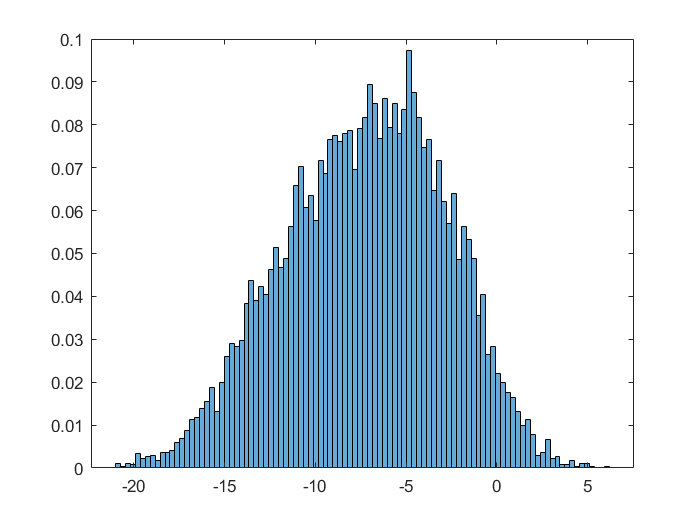
\includegraphics[scale=1]{pictures/2/histogram}
\caption{Хистограм процењене густине вероватноће}\label{fig:WaldoHisto}
\end{figure}


\begin{lstlisting}[caption={Процена условног h},label={fun:estH}]
function [expValCond, hApprox] = condProbDiscApprox(P11, P12, P21, P22, M11, M12, M21, M22, S11,...
                                                    S12, S21, S22)
num_points = 10000;
X1Approx = gausianMultimodalGenerate(P11, P12, M11, M12, S11, S12, num_points);
m = size(X1Approx, 1);
hApprox = zeros(m, 1);

for i = 1 : m
    tempInput = X1Approx(i, :)';
    f1Approx = gausianMultimodal(tempInput, P11, P12, M11, M12, S11, S12);
    f2Approx = gausianMultimodal(tempInput, P21, P22, M21, M22, S21, S22);
    hApprox(i) = log(f2Approx) - log(f1Approx);
end

[condProb, bins] = histcounts(hApprox, 100, 'Normalization', 'pdf');

expValCond = 0;
step = bins(2) - bins(1);
for i = 1 :  length(condProb)
    x = (bins(i) + bins(i + 1)) /2;
    expValCond = expValCond + x * condProb(i) * step;
end

end

\end{lstlisting}

\begin{figure}[htb!]\caption{Графици зависности}
\begin{subfigure}{.6\textwidth}
\centering
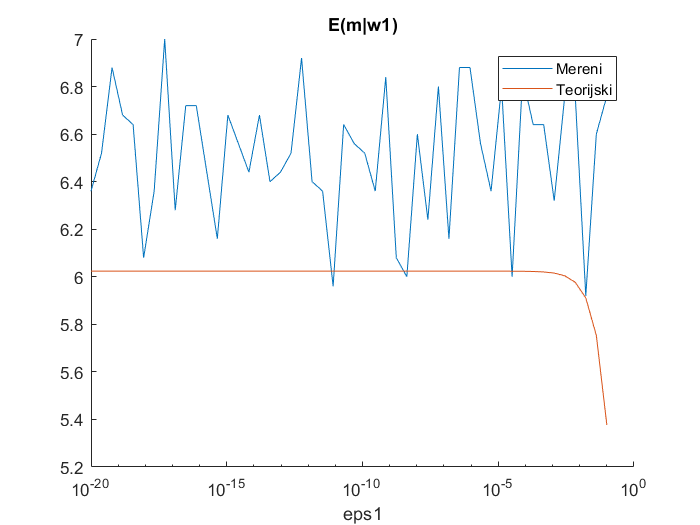
\includegraphics[width=1\linewidth]{pictures/2/WaldoE1}
\caption{$\varepsilon_2 = 10^-20$, зависност у односу на $\varepsilon_1$}\label{pic:eps1Dep}
\end{subfigure}
\begin{subfigure}{.55\textwidth}
\centering
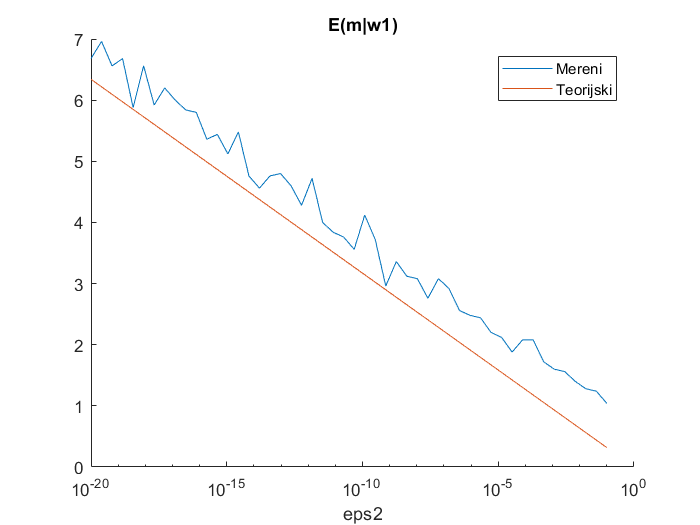
\includegraphics[width=1\linewidth]{pictures/2/WaldoE2}
\caption{$\varepsilon_1 = 10^-20$, зависност у односу на $\varepsilon_2$}\label{pic:eps2Dep}
\end{subfigure}
\end{figure}

Са последње две слике се  уочава да очекивани број одбирака из прве класе за доношење одлуке  зависи од вероватноће грешке другог типа, док вероватноћа грешке првог типа скоро па нема утицај. Аналогно за другу класу, потребан број одбирака из друге класе  зависи од $\varepsilon_1$, док скоро уопште не зависи од $\varepsilon_2$